%%%%%%%%%%%%%%%%%%don't forget if needed %%%%%%%%%%%%%%%%%%%%%
%\section[toc version]{title version%
%              \sectionmark{head version}}
%\sectionmark{head version}
%%%%%%%%%%%%%%%%%%%%%%%%%%%%%%%%%%%%%%%%%%%%%%%%%%%%%%%%%%%%%%
\def\titcourt{Numerical simulation of natural convection flow}
\def\titlong{Numerical simulation of natural convection flow}
%%%%%%%%%%%%%%%%%%%%%%%%%%%%%%%%%%%%%%%%%%%%%%%%%%%%%%%%%%%%%%%%
\chapter[\titlong]{\titlong%
              \chaptermark{\titcourt}}
\chaptermark{\titcourt}
\label{chap-NATCONV}
%%%%%%%%%%%%%%%%%%%%%%%%%%%%%%%%%%%%%%%%%%%%%%%%%%%%%%%%%%%%%%%%
%%%%%%%%%%%%%%%%%%%%%%%%%%%%%%%%%%%%%%%%%%%%%%%%%%%%%%%%%%%%%%%%

We first focus on the capability of our code to deal with natural convection flow in enclosures.
The richness of studies on internal natural convection flow allows us to validate the Navier-Stokes-Boussinesq solver in the fluid part.
A large number of benchmark solutions exists in the literature for natural convection induced by temperature difference since it is central in a long list of engineering (circulations in building applications, double-wall insulations, solar collectors, etc.) and geophysical systems.
%The influence of the geometric aspect ratio, the inclination, the heating orientation (if we heat from the side or from below), the $\Ray$ number have been widely studied.
%It is indeed well-known that the heat transfer is completely different from tall enclosure or shallow enclosure limits. 
%In one case, the heat transfer is dominated by conductive transfer (such as double-wall insulations) and in the second case the heat transfer is dominated by the presence of vertical layer.
In this chapter, we are interested by natural convection of fluid in a square cavity differentially heated from the vertical walls.
%in which a fluid recirculation exists because of buoyancy forces.
The fluid temperature rises and its density decreases along the heated wall, convecting the fluid up to the point where it reaches the cold wall, where the reverse process occurs. 
This two simultaneous opposing effects create a recirculation cell within a stationary zone in the center.

We solve the system of eqs. (\ref{eq-qmvt}) - (\ref{eq-energ}), with $A(\theta) = 0$ in the momentum equation and $S(\theta) = 0$ in the energy equation.
Linear and non-linear expressions of the buoyancy force $f_B(T)$ in the Boussinesq approximation (\ref{eq-energie-enth-model}) are investigated, by simulating the natural convection of air and the natural convection of water.
Natural convection of water exhibits actually a non-linear variation of the density with a maximum value around $T=4^o C$ while a linear variation is generally assumed for the natural convection of air in the Boussinesq approximation.
We consider a square enclosure of height $H$. 
Physical properties of air and water are listed in Tab. \ref{tab-param-phys-air}.
\begin{table}[ht!]
   \begin{center}
      \begin{tabular}{*{8}{cl}}
         
        & $\rho$ &$ \mu$ & $c_p $ & $k$ & $\alpha $ & $\beta$ \\
        & kg/m$^3$& kg/(m s) & J/(kg K) & W/(m K) & m$^2$/s & 1/K \\
         \hline
        Air & 1.177 & 1.85 $\cdot 10^{-5}$  & 1006 & $0.0262$ & $2.22 \cdot 10^{-5}$ & $3.4 \cdot 10^{-3}$ \\
        Water & 999.84 & 1.003 $\cdot 10^{-3}$  & 4182 & $0.578$ & $1.33 \cdot 10^{-7}$ & $6.91 \cdot 10^{-5}$
      \end{tabular}
   \end{center}
   \caption{Physical parameters of air and water at $T = 300K$ used in our simulations. $\Pr = 0.71$ (for air) and $\Pr = 6.99$ (for water).}
   \label{tab-param-phys-air}
\end{table}

\noindent Isothermal boundary conditions are applied to the vertical walls and adiabatic boundary condition to the upper and lower walls.
Quantitative and qualitative validations are carried out as following:
\begin{enumerate}[label=(\roman*)]
\item Natural convection of air in a two dimensional square cavity: velocity profile along symmetry lines, the maximum value of $u_{max}$ at mid-domain($x=0.5$) and location $Y$ of this maximum  are compared with the spectral-accurate simulations by \cite{LeQuere91} in Sec. \ref{sub-diff-heated}, 
\item Natural convection of air in a 2D square cavity with inner heated square obstacle: transversal velocity profile along the  horizontal symmetry lines is compared with numerical results of \cite{Raluca2013} 
in sec. \ref{sub-2D-OBSTACLE}, 
\item Natural convection of water in a 2D square cavity: Temperature profile along the horizontal symmetry line is compared with the numerical results of \cite{Kowalewski-2003} in sec. \ref{sec: natconv-water}.
%\item Natural convection of air in a cube: the temperature field is qualitatively compared with numerical results of \cite{Wakashima-2004} and a comparison between ffddm and the sequential algorithm is given in 
%sec. \ref{sec: natconv-air-3D},
%\item Natural convection of air in a cube with a cubic heated obstacle is presented in sec. \ref{sub-OBSTACLE-3D}.
\end{enumerate}

\section{Natural convection of air in a two dimensional square cavity}\label{sec: natconv-air-2D}
We start by testing the Newton algorithm (\ref{eq-newton-C1}) by investigating simulations with linear expression of $f_B(\theta)$ as presented in eq. (\ref{eq-RePr}).
The classical problem of the thermally driven square cavity with adiabatic top and bottom walls is of interest.
We consider a cavity of height $H = 0.1$m, initially filled with motionless air with a linear distribution of the temperature. 
The dimensionless parameters describing the investigated configuration are based on the fluid properties presented in tab. (\ref{tab-param-phys-air}), mainly $\Pr = 0.71$.
Three $\Ray$ numbers are computed $Ra = 10^4, 10^5, 10^6$, and
the characteristic scales of the problem defined in eq. \ref{eq-adim} are:
\begin{equation} \label{eq-scale-air}
	L_{ref} = H, \quad T_{ref} = \frac{T_h + T_c}{2},
\end{equation}
and
\begin{equation} \label{eq-scaling-3}
   V_{ref} = \frac{\nu_l}{H} \sqrt{\frac{Ra}{Pr}} 
   \quad \Longrightarrow \quad t_{ref} = \frac{\nu_l}{H^2} \sqrt{\frac{Pr}{Ra}} 
   \quad \Longrightarrow \quad \Rey = \sqrt{\frac{Ra}{Pr}}.
\end{equation} 
The left wall is heated with dimensionless hot temperature $\theta_h = 0.5$ and the right wall is cooled with $\theta_c = -0.5$ (resulting from Eq. \ref{eq-scale-air}). 
A no-slip velocity boundary condition ($\vec u = 0$) is used.

It has been shown by \cite{LeQuere91} that the solution of the 2-D Boussinesq equation in this configuration becomes unsteady at $Ra = 10^{8.5}$.
Therefore, steady state can be achieved for the chosen Rayleigh numbers.

The unsteady and steady Navier-Stokes-Boussinesq equations are simulated.
The unsteady case is computed until the steady state with a single convection cell is reached, with a numerical tolerance of $10^{-9}$.
Besides, the steady case is performed using Rayleigh number continuation:
a smaller value of the Rayleigh number is set initially, and is then increased smoothly until reaching the correct value.
At each stage, the computation starts from the solutions obtained from the previous Rayleigh number simulation.

Two cases are carried out: {\it i)} a differentially heated square cavity and {\it ii)} a differentially heated cavity with inner heated obstacle.
For each of them, the horizontal and the vertical velocity profiles $u(y)$ and $v(x)$ at mid-domain ($y=0.5$ and $x=0.5$ respectively) are plotted and compared with numerical result by \cite{LeQuere91} and \cite{Raluca2013}. 
Moreover, for {\it i)} the maximum value $u_{max}$ and its location $Y$ are accurately compared with the solutions obtained by spectral accurate simulations by \cite{LeQuere91}.

\subsection{Differentially heated square cavity} \label{sub-diff-heated}

\begin{figure}[!h]
	\begin{center}
		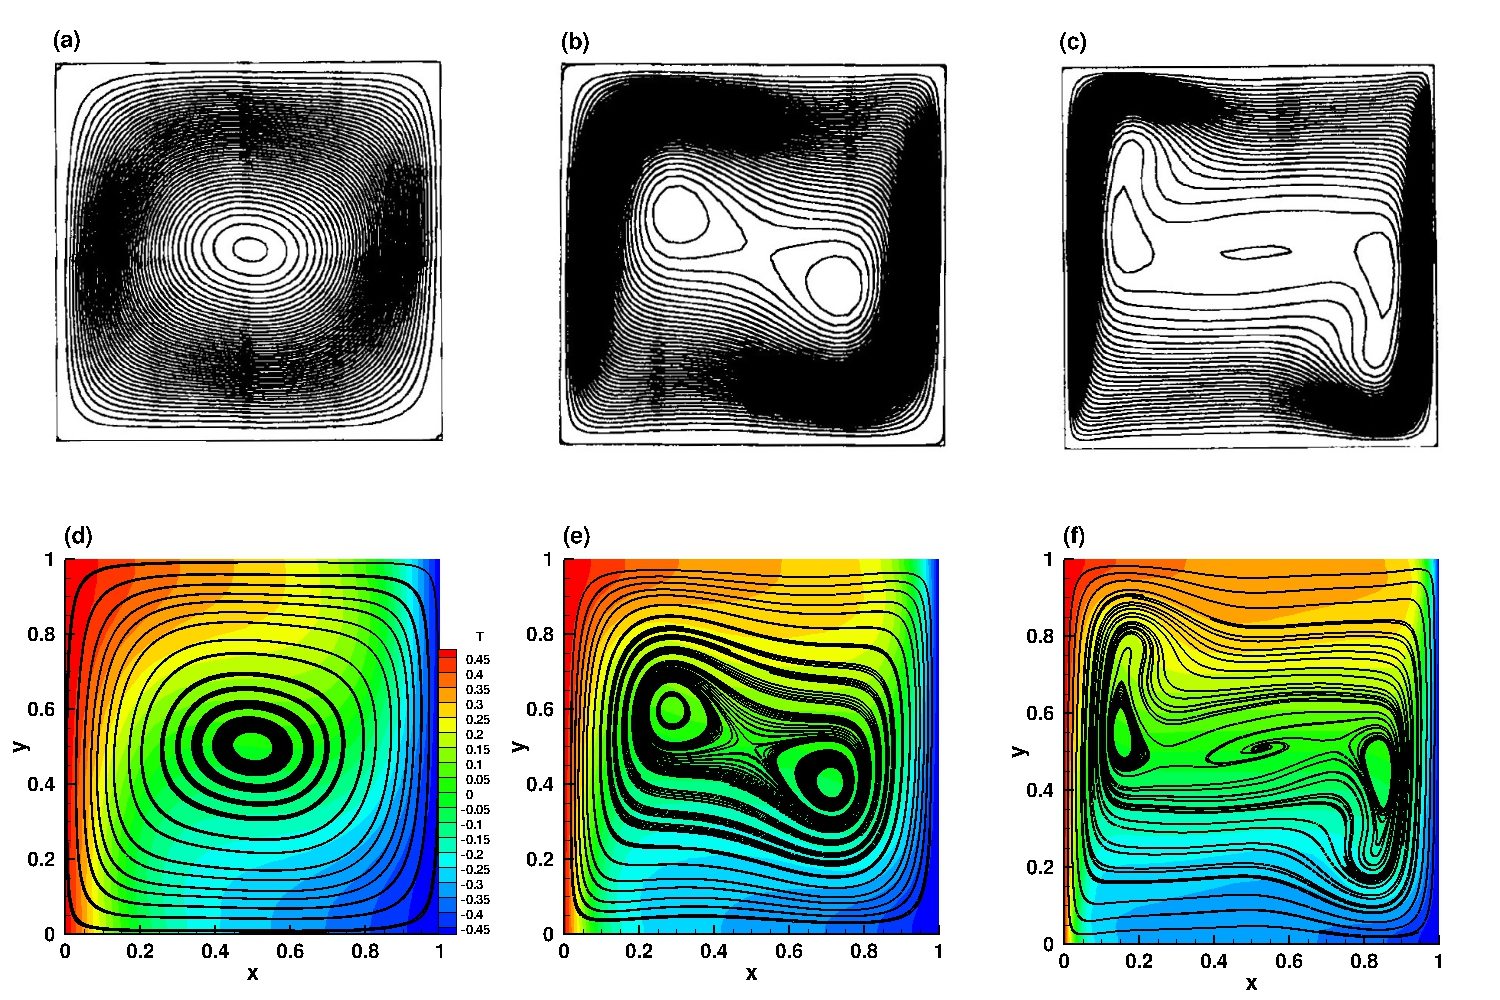
\includegraphics[width=0.98\textwidth]{\figpath/Fig_cap_natconv/NATCONV_air_valid-WS} 
	\end{center}
	\caption{Natural convection of air for $Ra = 10^4$ (a and d), $Ra = 10^4$ (b and e), and $Ra = 10^6$ (c and e), and $\Pr = 0.71$. Temperature fields and streamlines at the steady state. Panels (a) to (c) correspond to the benchmark solution of \cite{Wakashima-2004}. Panels (d) to (f) show our numerical results.}
	\label{fig-natconv-field}
\end{figure}

All computations in this section are performed with a fixed triangular mesh, generated by the Delaunay algorithm starting with \texttt{nbseg = 80} points on each side of the square.

Fig. \ref{fig-natconv-field} gives a comparison of the current simulation with the numerical results of \cite{Wakashima-2004}, who
used a fourth-order finite difference method for spatial discretization and third-order backward finite difference scheme for time integration.
Our results match qualitatively well with the Benchmark solution.
The natural convection in the cavity is clearly enhanced when the $\Ray$ number is increased.
A single convection cell is observed in the center of the cavity for $\Ray = 10^4$ (Fig. \ref{fig-natconv-field}d) indicating that the heat transfer is dominated by the bulk heat transfer.
Figs. \ref{fig-natconv-field}e and \ref{fig-natconv-field}f however exhibit stronger convection with more convection cells, meaning that the heat transfer is boundary layer heat transfer

Fig. \ref{fig-T1-prof} illustrates a comparison of the horizontal (Fig. \ref{fig-T1-prof}a) and the vertical (Fig. \ref{fig-T1-prof}b)  profiles of the velocity with data extracted from  \cite{LeQuere91} for each of the three computed $\Ray$ numbers.
Results from \cite{LeQuere91} are represented by solid lines and the current simulation by symbols.
A very good agreement can  be noticed for each of the three Rayleigh numbers.

\begin{figure}
	\begin{center}
		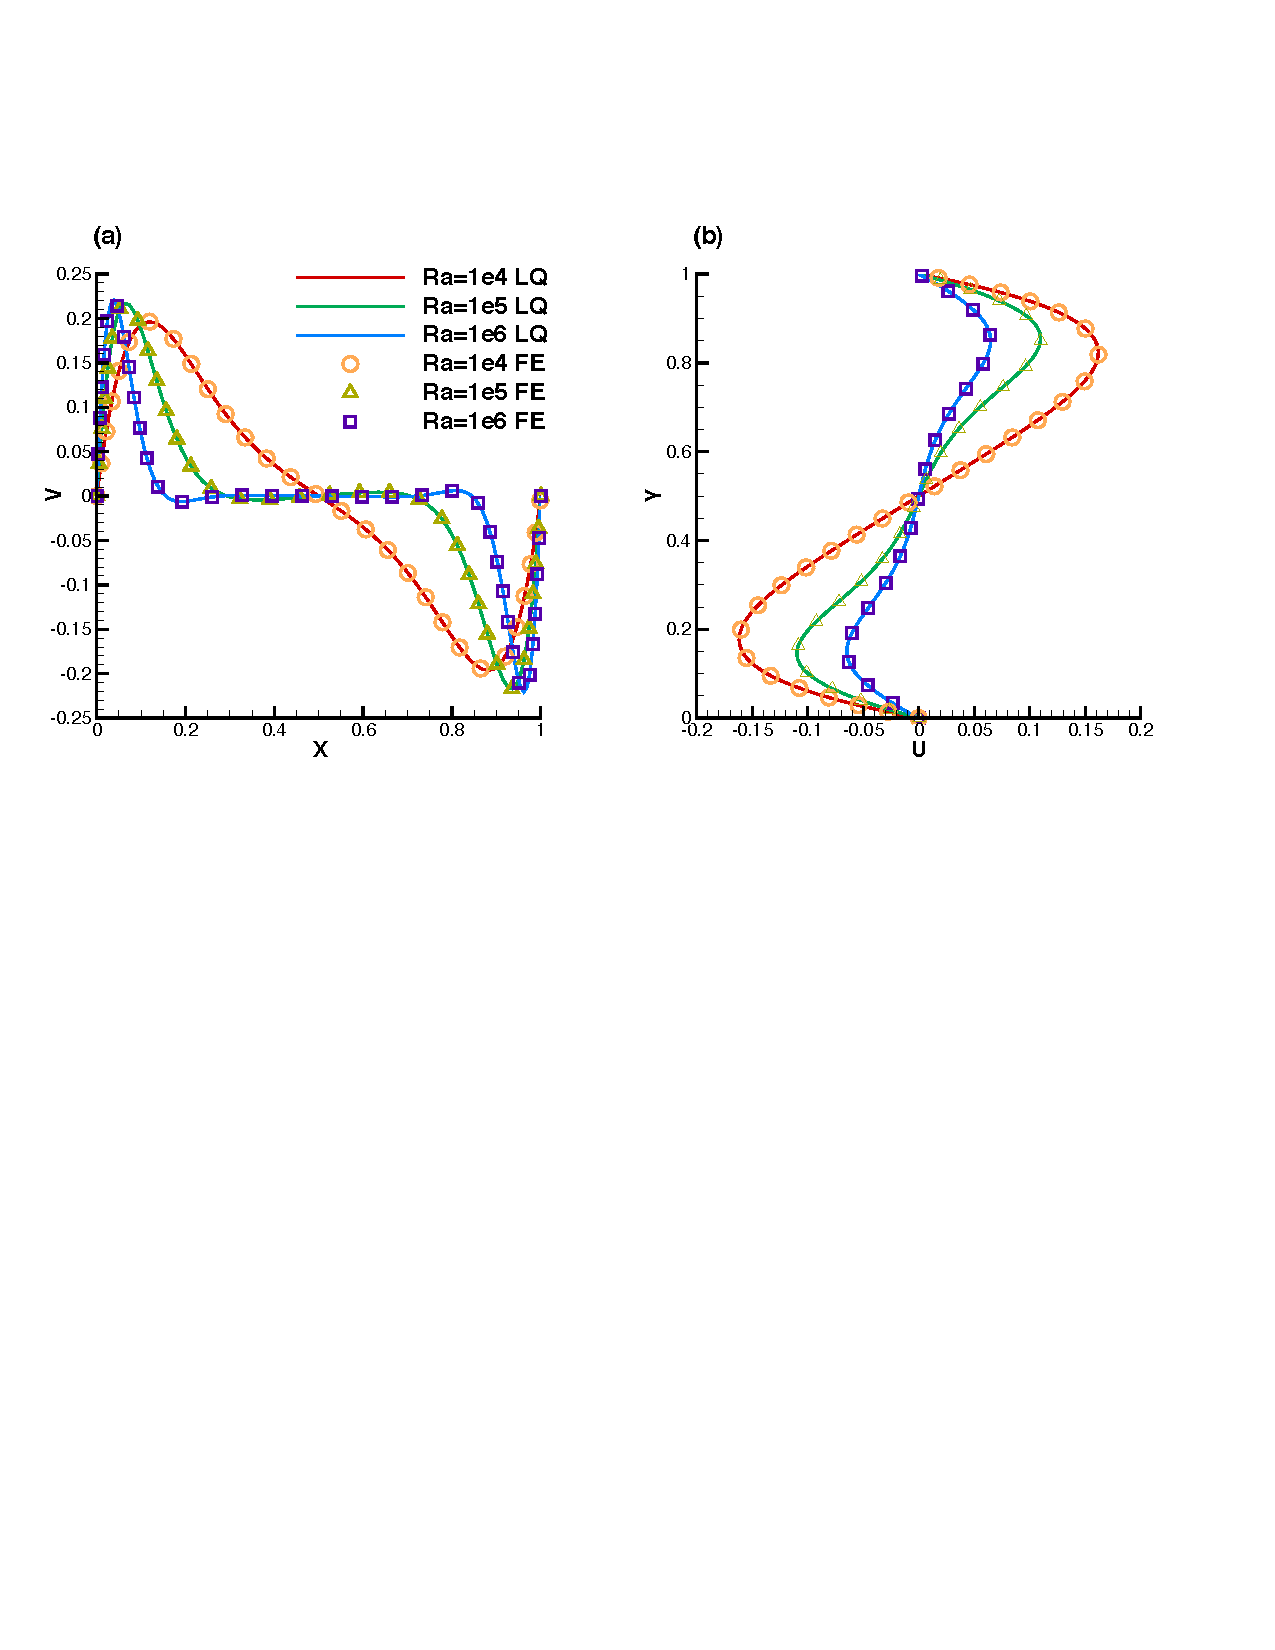
\includegraphics[width=0.98\textwidth]{\figpath/Fig_cap_natconv/Validation_Uprofile_LQ} 
	\end{center}
	\caption{Natural convection of air in a differentially heated cavity for $Ra$ ranging from $10^4$ to $10^6$ and $\Pr = 0.71$. (a) Transversal velocity profile along the  horizontal symmetry lines. (b) Longitudinal velocity profile along the vertical symmetry lines. Numerical results obtained using the present Newton method (symbols) with a mesh resolution of $M=80$; comparison with the spectral-accurate simulations by \cite{LeQuere91} (solid lines).}
	\label{fig-T1-prof}
\end{figure}

The influence of the imposed temperature difference $\delta T$ on the boundary layers are well illustrated in Fig.  (\ref{fig-T1-prof}).
Eq. (\ref{eq-corr-Low-Pr}) indicates a decreasing thickness of the boundary layer for an increasing value of $\Ray$. 
For $\Ray = 10^6$ a viscous boundary layer with a dimensionless thickness of order of $\delta_\nu \sim 0.02$ should be present close to the vertical walls.
Accordingly, the mesh resolution should allow to capture these structures.
A mesh convergence analysis shows a reasonable relative error (lower than $3\%$) from a $80 \times 80$ grid resolution.
Also, from $\Ray = 10^5$ the fluid in the core of the cavity is relatively stagnant and thermally stratified.

Tab. \ref{tab-valid-natconv} offers a quantitative assessment of the accuracy of the present Newton method. 
The values of $u_{max}$  and its location $Y$ are compared to reference values from \cite{LeQuere91}. 
The Newton method gives results very identical to reference values, with a relative difference less than $0.01 \%$ for the steady and the unsteady codes. 
The characteristics-Galerkin method is less accurate, but still offers reasonable agreement with reference values, within 2$\%$ relative error. 
We also recall that the characteristics method needs a very small time step for refined meshes ($\delta t = 8\cdot 10^{-5}$ for \texttt{nbseg = 80}), while the Newton method allows larger time steps ($\delta t = 1$ for \texttt{nbseg = 80}). % and consequently, converges faster to a steady state.
%It is worth noting, that the steady and the unsteady codes provide quasi-identical results.
\begin{table}%[!h]
	\begin{center}
		\begin{tabular}{|l|c|l|l|}
			\hline
			\multicolumn{2}{|l|}{Run} & $u_{max}$ at x=$0.5$ (error) & $Y$ (error) \\
			\hline
			Reference values & spectral & 0.0648344           & 0.850 \\ \hline
			Char-Galerkin       &$M=80$ & 0.0662229 (2.14 $\%$) & 0.856160 ( 0.72 $\%$) \\ \hline
			\cite{dan-2014-JCP}              &$M=80$ & 0.0650082 (0.26 $\%$) & 0.849906 ( 0.01 $\%$) \\ \hline
			Newton (Steady)        &$M=80$ & 0.0648297 (0.007 $\%$) & 0.850394( 0.05 $\%$) \\ \hline
			Newton (Unsteady)        &$M=80$ & 0.0648296 (0.007 $\%$) & 0.850532 ( 0.06 $\%$) \\ \hline
		\end{tabular}
	\end{center}
	\caption {Natural convection of air in a differentially heated cavity for $Ra = 10^6$ and $\Pr = 0.71$. Maximum value $u_{max}$ of the horizontal velocity profile at mid-domain ($x=0.5$) and location $Y$ of this maximum. Comparison to reference values by \cite{LeQuere91}.}
	\label{tab-valid-natconv}
\end{table}

Finally, we compare the average Nusselt number at the left vertical wall with the reference values of \cite{de1983natural} and \cite{LeQuere91}.
From the viewpoint of an engineer, the most important characteristic of the flow is probably the rate of heat  transfer across the cavity.
In the next chapters, the Nusselt number will be largely used to compare the optimized configuration of a PCM either for melting or solidification.
It is thus essential to ensure about the accuracy of the computed value of this parameter.
$N\!u$ is calculated as defined in Eq. \ref{eq-def-Nu}.
The comparison with \cite{de1983natural} is summarized below in Tab. \ref{tab-Nu-natconv}:
\begin{table}[ht!]
   \begin{center}
      \begin{tabular}{*{4}{cl}}
         
       $\Ray$ & $10^4$ &$ 10^5$ & $10^6 $ \\
         \hline
        \cite{de1983natural} & 2.245 & 4.523  & 8.927 \\
        \cite{LeQuere91} & - & - &  8.8252 \\
        Present simulation & 2.2448 & 4.5217  & 8.8252 \\
      \end{tabular}
   \end{center}
   \caption{Average Nusselt number on the vertical boundary of the cavity at $x=0$. Comparison with \cite{de1983natural} and \cite{LeQuere91} for $Ra = 10^4$ to $10^6$.}
   \label{tab-Nu-natconv}
\end{table}

Excellent agreement with \cite{de1983natural} is obtained for each of the three $\Ray$ numbers, with a relative error lower than $0.01$.
It is important to note that we have exactly the same computed value of the Nusselt number as \cite{LeQuere91}.
Also, the comparison with a P$_1$ discretization of the temperature have also been carried out and larger differences between \cite{de1983natural} and \cite{LeQuere91} was observed.

\subsection{Differentially heated cavity with inner heated square} \label{sub-2D-OBSTACLE}

\begin{figure}
	\begin{center}
		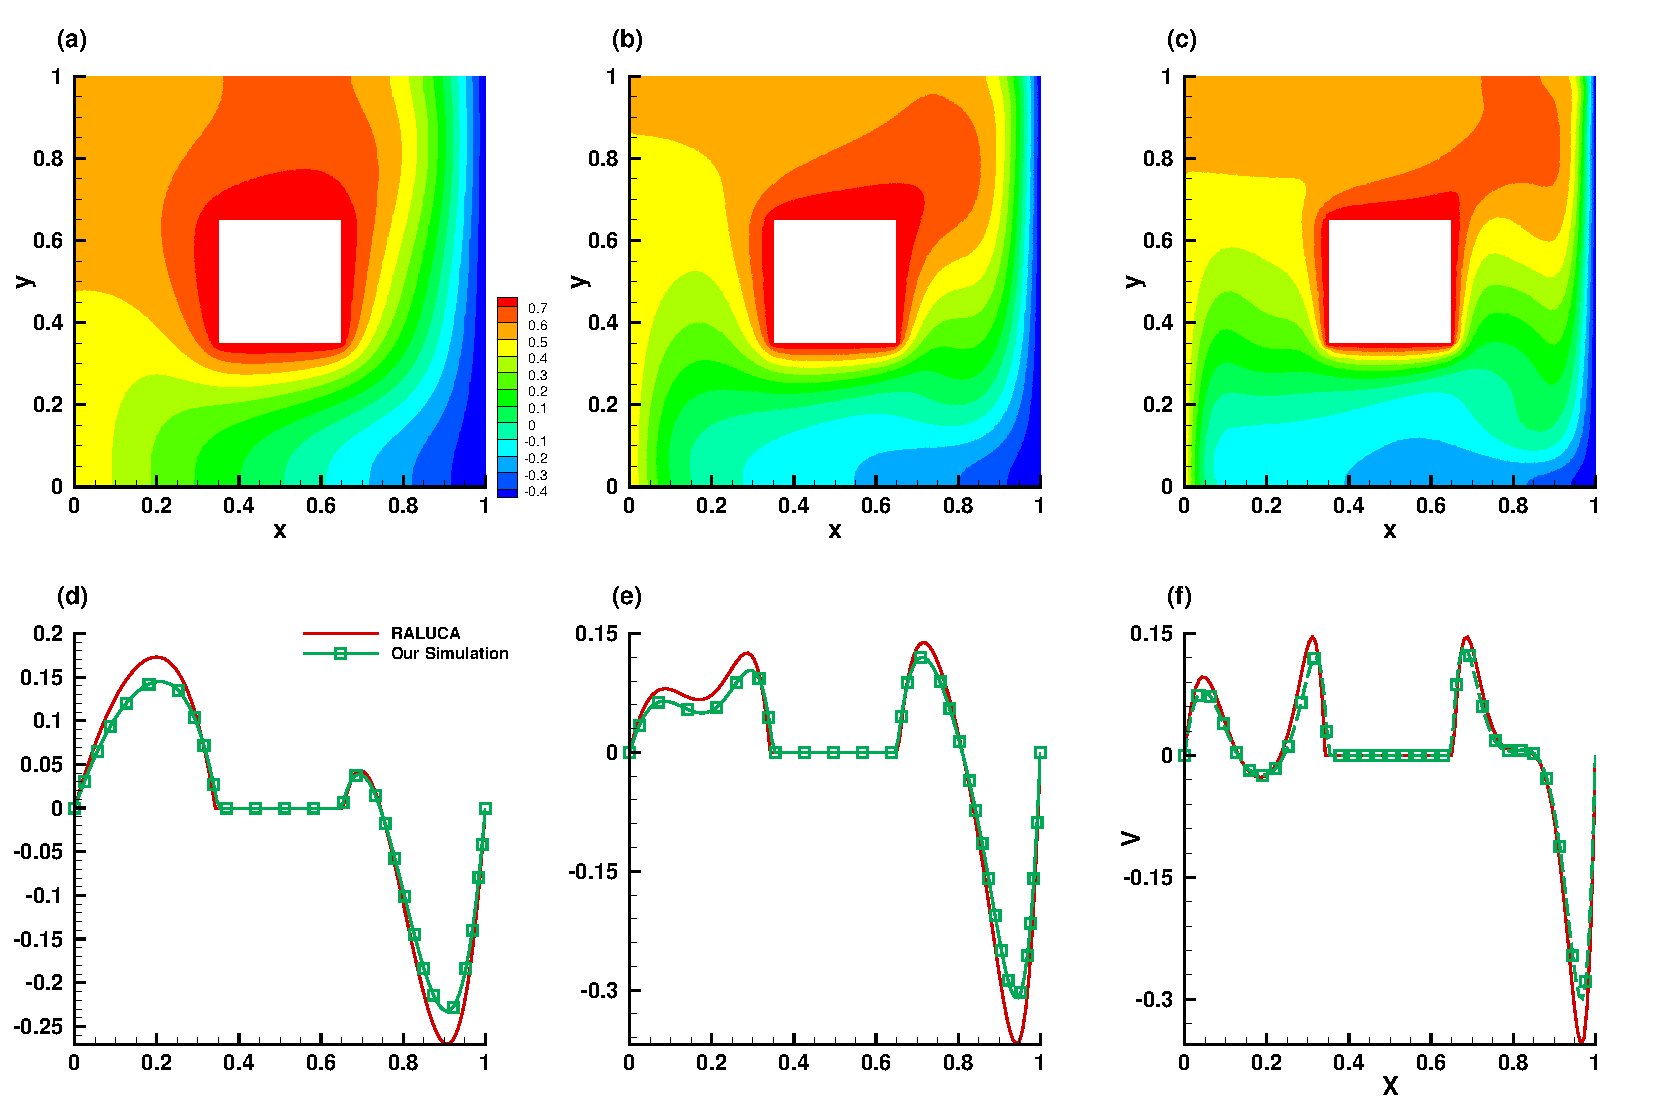
\includegraphics[width=\textwidth]{\figpath/Fig_cap_natconv/STA_validation_obstacle_2} 
	\end{center}
	\caption{Natural convection of air in a differentially heated cavity with inner heated square for $Ra = 10^6$. Temperature field (a) and transversal velocity profile along the  horizontal symmetry lines (b). Results obtained using the present Newton method (red solid line), with mesh resolution $M=80$; comparison with the finite difference code of \cite{Raluca2013}.}
	\label{fig-obst-2D}
\end{figure}

Thermally driven cavity including heated square obstacle is computed in this section.
We consider the same configuration presented in sec. \ref{sub-diff-heated} and a square involving isothermal boundary condition is added between the initial set up.
This kind of basic configuration could be representative of telecommunication outdoor cabinet applications, in which the use of passive cooling solutions have begun to be more and more investigated.
Indeed, inside an outdoor cabinet, electronic equipments generate heat when active and the study of the flow structures within the enclosure have attracted some considerations at the example of the experimental and numerical study of \cite{Raluca2013}.
Simplified model of cavity with rectangular heated obstacles have been investigated by \cite{Raluca2013} and will be reproduced in this section to test the robustness of our numerical algorithm.

A linear distribution of the temperature is imposed initially in the motionless air inside the cavity.
The obstacle is maintained at a dimensionless hot temperature $\theta_h = 0.8$ with a no-slip boundary condition for the velocity.
The solutions for $Ra = 10^4$, $Ra = 10^5$, $Ra = 10^6$ and $Pr = 0.71$ are compared with the result obtained by \cite{Raluca2013} who used an immersed boundary method with a FD code using high order schemes for time and spatial discretization.

The temperature distribution in the cavity when the steady-state is reached, for each of the three $\Ray$ number computed, are shown in panels (a) to (c) of Figs. \ref{fig-obst-2D}.
The temperature gradient gives rise to a clockwise circulation and when $\Ray$ is increased, vertical thermal boundary layers form distinctly along the differentially heated sidewalls and the obstacle.
Consequently, 
higher is the Rayleigh number the more the hot temperature in the center of the domain is advected by the natural convection flow into the cold part of the cavity. 
Worth noting is the fact that at $\Ray = 10^6$ in panels (c) and (d), a stagnant fluid with a stratified temperature forms in a small portion of the fluid between the cold wall and the obstacle.

A more accurate validation is given in panels (d) to (f) of Fig. (\ref{fig-obst-2D}).
The transversal velocity profiles along the x-axis are plotted and compared with the numerical data of \cite{Raluca2013} for each of the three $\Ray$ number investigated. 
A good agreement can be observed with a relatively small differences between the extremum of the velocity while the trends of the velocity profile match well.

We have demonstrated in this part that the proposed Newton method offers an efficient way to solve the Navier-Stokes-Boussinesq system of equations for natural convection of air evolving a linear expression of $f_B(\theta)$.
A further difficulty will be introduced in the next section when a non-linear expression of the body force is defined since natural convection of water is of interest.
%We can conclude from this section that the proposed Newton method offers an efficient way to solve the Navier-Stokes-Boussinesq system of equations for natural convection. After this validation, we test in the following section the capability of the method to deal with phase-change, introducing nonlinearity in the momentum and the energy equations.

\section{Natural convection of water in a two dimensional square cavity}\label{sec: natconv-water}
We investigate in this section the natural convection of water in a differentially heated cavity. 
A further difficulty is introduced compared to the previous validations by taking into account non-linear variation of the density in the buoyancy force.
Pure water involves actually non-linear density variation for $T< \celsm{10.2}$ with a maximum at $T_m= \celsm{4.0293}$. 
We use below the following density-temperature relationship  proposed in \cite{Gebhart1977}:
\begin{equation}\label{eq-dens-nonlin}
\rho(T)=\rho_m \left(1 - w \left|T - T_m\right|^q\right),
\end{equation}
with $\rho_m=999.972$ [kg/m$^3$], $w=9.2793\cdot 10^{-6}$ [($^\circ C)^{-q}$], and $q=1.894816$.
The bouyancy term $f_B = g(\rho_\vref-\rho)/\rho_\vref$ appearing in eq. (\ref{eq-momentum-conserv})  becomes after scaling:
\begin{equation}
f_B(\theta) = \frac{\Ray}{\Prd \, \Rey^2} \frac{1}{\beta \delta T}\, \frac{\rho(\theta_f)-\rho(\theta)}{\rho(\theta_f)},
\label{eq-fBnonlin}
\end{equation}
where $\beta=(1/\rho_m) \left(d\rho/dT\right)$ is the thermal expansion coefficient with the value \cite{Scanlon2004} $\beta=6.91 \cdot 10^{-5}$ [(K)$^{-1}$].

We simulate a differentially heated cavity of height $H = 0.38 m$ filled with liquid pure distilled water.
This problem was investigated experimentally and numerically in \cite{Giangi-2000,Kowalewski-1999,Kowalewski-2003}.
The height $H$ of the cavity is considered as a length scale of the problem $L_{ref} = H$. 
We choose $T_{ref} = T_h - T_c = 10 K$ in order to compare our simulation with the numerical results of \cite{Kowalewski-2003},
and define the following scaling:
\begin{equation} \label{eq-def-scal-1}
   V_{ref} = \frac{\nu_l}{H} 
   \quad \Longrightarrow \quad t_{ref} = \frac{\nu_l}{H^2}
   \quad \Longrightarrow \quad \Rey = 1.
\end{equation} 
The non-dimensional parameters describing the problem result from the physical properties of water in Tab. \ref{tab-param-phys-air}: $\Ray=2.518084\cdot 10^{6}$ and $\Pr=6.99$. %  (see also \cite{Kowalewski-2003} for physical details). % and $\Ste = 6.99$.

The initial temperature is linearly distributed with a hot temperature $\theta_h =1$ at the left wall and a cold temperature $\theta_c=0$ at the right wall. %, corresponding to dimensionless thermal boundary condition $\theta_h = 1$ and $\theta_c = 0$. 
The top and the bottom of the cavity are adiabatic and no-slip boundary condition $\vec u = 0$ is used for the velocity.

The Temperature field of the steady state is presented in Fig. (\ref{fig-T1w-isoT}a).
Unlike the natural convection of air, in which two distinct boundary layers along the vertical walls and a stagnant and thermally stratified fluid in the core of the fluid flow were observed, an anomalous variation of the temperature is pointed out around the iso-line $\theta = 0.4$ for the natural convection of water.
This anomalous thermal variation of water density, is clearly discernible in the streamline of the steady flow in Fig. (\ref{fig-T1w-isoT}b).
Two recirculating zones are formed in the flow: a lower (abnormal) recirculation  in the vicinity of the cold wall where $\theta<\theta_m$ and an upper (normal) one where the density decreases with temperature ($\theta>\theta_m$).

Accounting for the foregoing comments, a greater mesh resolution should be applied around $\theta_m$.
We define thus a P$_1$ function $\Phi(\theta)$ defined by the following hyperbolic-tangent function similar to eq. (\ref{eq-Stanh}):
\begin{equation}
\Phi(\theta) =  \frac{1}{2}\left\{
1 + \tanh\left(\frac{\theta_m-\theta}{R_{\Phi}}\right)
\right\},
\label{eq-Stm}
\end{equation} 
with $R_{\Phi}=0.02$. 
The function $\Phi(\theta)$ and the two components of the velocity are used to compute the metric for the adaptivity.
$\Phi(\theta)$ is used to track $\theta_m$ and the velocity allows to refine the boundary layer region.
To reduce the reduce the impact of the interpolation on the global accuracy, since our algorithm is optimized to afford the mesh refinement every time step, we use both $\Phi(\theta^n)$ and $\Phi(\theta)^{n+1}$ in the adaptivity procedure.
The final mesh is displayed in Fig. (\ref{fig-T1w-isoT}c).
The mesh is clearly refined along the line $\theta = \theta_m$ where  the structure and the extent of the two recirculating zones should be captured and along the vertical walls where the heat transfer is dominated by the boundary layer transfer.
Furthermore, as expected in the relatively stagnant fluid region, a coarser mesh is applied.

A more accurate comparison of the temperature profile along the horizontal symmetry line is given in Fig. \ref{fig-T1w-isoT}b. 
The temperature profile $\theta(x)$ along the horizontal symmetry line of the cavity is in good agreement with the numerical results   of \cite{Kowalewski-2003} obtained with FV and FD codes (FLUENT and FRECONV3V), commonly used in the heat transfer community. Differences are visible in the vicinity of the maximum density line, region where our mesh is well refined to capture the separation line between the two recirculation zones. It should be noted that the FLUENT simulations in \cite{Kowalewski-2003} are performed with a fixed uniform grid with $380\times380$ nodes, while our adapted grid has only 8751 vertices (17257 triangles).

\begin{figure}
	\begin{center}
		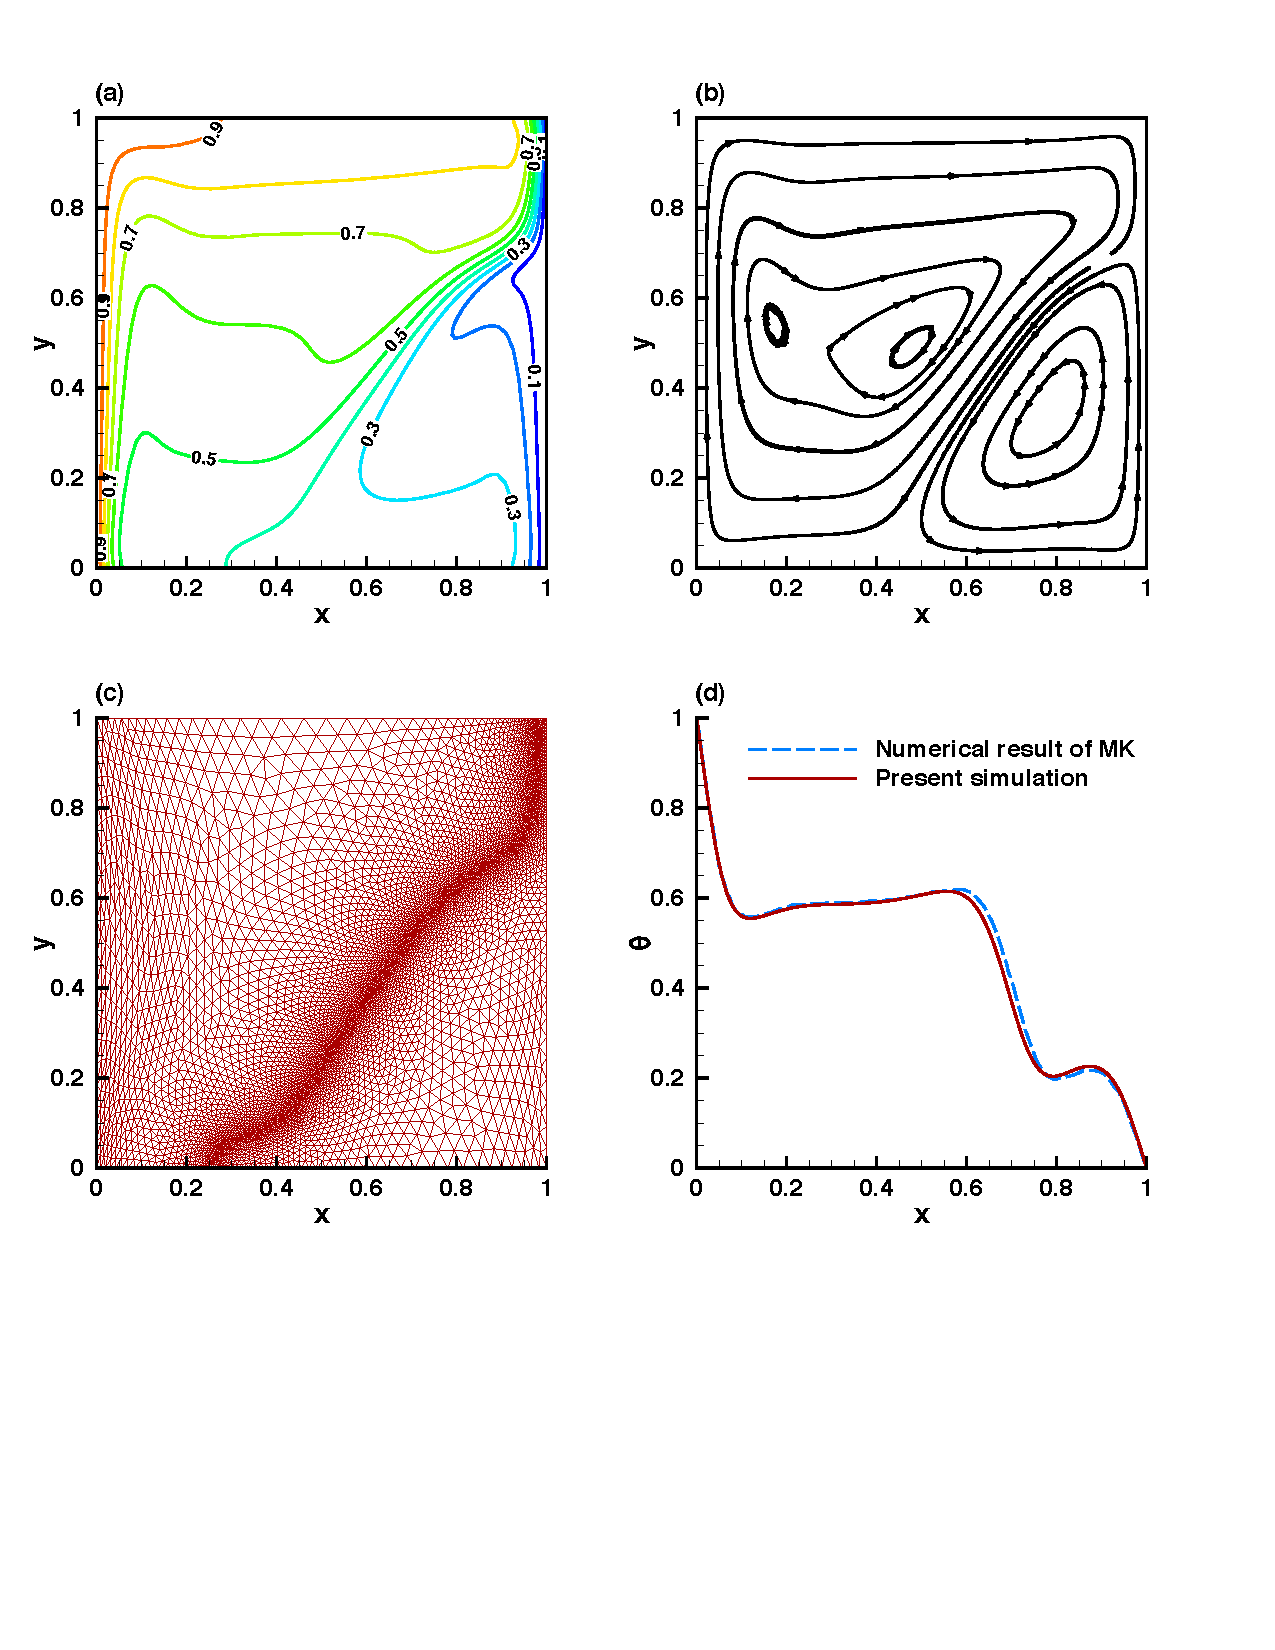
\includegraphics[width=0.98\textwidth]{\figpath/Fig_cap_natconv/WATER_convec_valid}
	\end{center}
	\caption{Natural convection of water in a differentially heated cavity with non-dimensional parameters: $\Ray=2.518084\cdot 10^{6}$ and $\Pr=6.99$. (a) iso-line of the temperature at the steady state. (b) Streamline of the steady flow. (c) Illustration of the mesh adaptivity: The mesh is refined along the dimensionless temperature iso-line $\theta = 0.4$ due to the density variation. (d) Temperature profile along the horizontal symmetry line. Comparison with the numerical results of \cite{Kowalewski-2003}.}
	\label{fig-T1w-isoT} % label should be placed after the caption
\end{figure}

We can conclude from Secs. (\ref{sec: natconv-air-2D}) and (\ref{sec: natconv-water}) that the developed Newton method is able to deal  efficiently with the two-dimensional Navier-Stokes-Boussinesq problem either with linear or non-linear formulations of the buoyancy force.
The natural convection of air including obstacle or not have shown very good agreement with the numerical solutions of \cite{LeQuere91} and \cite{Raluca2013}.
Excellent agreement with \cite{de1983natural} and \cite{LeQuere91} have also been observed for the value of the average Nusselt number at the heated wall. 
The challenging case of the natural convection of water have demonstrated the robustness of the 2D code. 
Good agreement with the numerical simulations of \cite{Kowalewski-2003} was noticed. 
The influence of the mesh adaptivity was clearly shown by the total grid number differences of order of eight between the present simulation and those of \cite{Kowalewski-2003} .
The refined mesh along the line $\theta_m$ have permitted to solve more accurately the structures and the extent of the two recirculating zones.
The next sections are now devoted to the three-dimensional simulations of natural convection of air using parallel algorithm.
%
%\newpage
%\section{Numerical simulation of the natural convection of air in a three-dimensional cavity using parallel agorithm}\label{sec: natconv-air-3D}
%
%\subsection{Natural convection of air in differentially heated cube cavity}
%We present in this section some 3D simulations using ffddm.
%
%The Prandtl number is $0.71$ and three Rayleigh numbers are considered:  $\Ray=10^4$, $\Ray=10^5$, $\Ray=10^6$. The walls are rigid and impermeable. The vertical walls at $x=0$ and $x=1$ are isothermal and have different temperatures $T_h=0.5$ and $T_c=-0.5$ respectively. The remaining walls are considered adiabatic. % Figure \ref{fig-3Dmesh} b) shows the present three dimensional grid.
% 
%Our result were obtained for uniform grids of $  40 \times 40 \times 40$ and is compared with \cite{Wakashima-2004} who used a forth order finite difference method, with a vorticity-stream function formulation with different uniform meshes of  $120 \times 120 \times 120 \times 10$ grid nodes. 
%This result obtained with sequential algorithm is also used to validate the 3D simulations using ffddm.
%
%Fig. \ref{fig-3DT} shows the temperature field for each of the three Rayleigh numbers $\Ray = 10^4$, $\Ray = 10^5$, $\Ray = 10^6$, at the mid section (y=0.5).
%On the left we display the numerical results of \cite{Wakashima-2004} and on the right ou results.
%The comparison with the benchmark solution exhibits a fairly good agreement.
%
%The parallel algorithm used with ffddm is compared with the sequential algorithm.
%$\mathcal{L}_2$-norm and $\mathcal{L}_\infty$-norm of the velocity and the temperature are computed and reported in Tab. \ref{tab-T1} for Rayleigh number varying from $10^4$ to $10^6$.
%The difference between both algorithm is of order of $10^{-6}$.
%Moreover, we do not observe a large variation of the error when the number of subdomains is increased.
%The number of subdomain vary from $28$ to $70$ for $1.8$ millions of unknown.
%
%\begin{table}[!h]
%	\begin{center}
%		\begin{tabular}{|*{6}{c|}}
%			\hline
%			 Ra & nb proc                     & $||u||_{2}$                        & $||u||_{\infty}$                & $||T||_{2}$              & $||T||_{\infty}$\\ \hline \hline
%			\multirow{4}{*}{$10^4$} & 28 & $1.12496 \cdot 10^{-6}$ & $3.1 \cdot 10^{-6}$ & $ 3.09966 \cdot 10^{-6} $ & $7 \cdot 10^{-6}$ \\% \hline
%			\cline{2-6}
%			& 42 & $1.53698 \cdot 10^{-6}$ & $5.1 \cdot 10^{-6}$ & $ 3.23352 \cdot 10^{-6} $ & $8 \cdot 10^{-6}$ \\ \cline{2-6} %\hline 
%			& 56 & $1.55576 \cdot 10^{-6}$ & $5.1 \cdot 10^{-6}$ & $ 3.4342 \cdot 10^{-6} $ & $8 \cdot 10^{-6}$  \\ \cline{2-6} %\hline
%			& 70 & $1.25622 \cdot 10^{-6}$ & $3.6 \cdot 10^{-6}$ & $ 3.56048 \cdot 10^{-6} $ & $8 \cdot 10^{-6}$ \\ \hline \hline
%			\multirow{4}{*}{$10^5$} & 28 & $1.73254 \cdot 10^{-6}$ & $6.1 \cdot 10^{-6}$ & $ 2.40467 \cdot 10^{-6} $ & $7 \cdot 10^{-6}$ \\% \hline
%			\cline{2-6}
%			& 42 & $2.84973 \cdot 10^{-6}$ & $7.78 \cdot 10^{-6}$ & $ 3.53003 \cdot 10^{-6} $ & $9 \cdot 10^{-6}$ \\ \cline{2-6} %\hline 
%			& 56 & $3.00832 \cdot 10^{-6}$ & $7.39 \cdot 10^{-6}$ & $ 4.17769 \cdot 10^{-6} $ & $1.1 \cdot 10^{-5}$  \\ \cline{2-6} %\hline
%			& 70 & $3.68118 \cdot 10^{-6}$ & $9 \cdot 10^{-6}$ & $ 4.70846 \cdot 10^{-6} $ & $1.2 \cdot 10^{-5}$ \\ \hline \hline
%			\multirow{4}{*}{$10^6$} & 28 & $6.61804 \cdot 10^{-6}$ & $1.826 \cdot 10^{-5}$ & $ 3.46504\cdot 10^{-6} $ & $1.1 \cdot 10^{-5}$ \\% \hline
%			\cline{2-6}
%			& 42 & $5.93966 \cdot 10^{-6}$ & $1.5 \cdot 10^{-5}$ & $ 3.98082 \cdot 10^{-6} $ & $1.2 \cdot 10^{-5}$ \\ \cline{2-6} %\hline 
%			& 56 & $7.05144 \cdot 10^{-6}$ & $1.9247 \cdot 10^{-5}$ & $ 5.0044 \cdot 10^{-6} $ & $2 \cdot 10^{-5}$  \\ \cline{2-6} %\hline
%			& 70 & $6.02152 \cdot 10^{-6}$ & $1.68 \cdot 10^{-5}$ & $ 4.50094 \cdot 10^{-6} $ & $1.8 \cdot 10^{-5}$ \\ \hline
%		\end{tabular}
%	\end{center}
%	\caption {3D differentially heated cavity. Comparison between sequential and ffddm algorithm for uniform grids of $40 \times 40 \times 40$ }
%	\label{tab-T1}
%\end{table}
%
%
%\begin{figure}%[!htbp]
%\begin{minipage}{\linewidth}
%\begin{center}
% {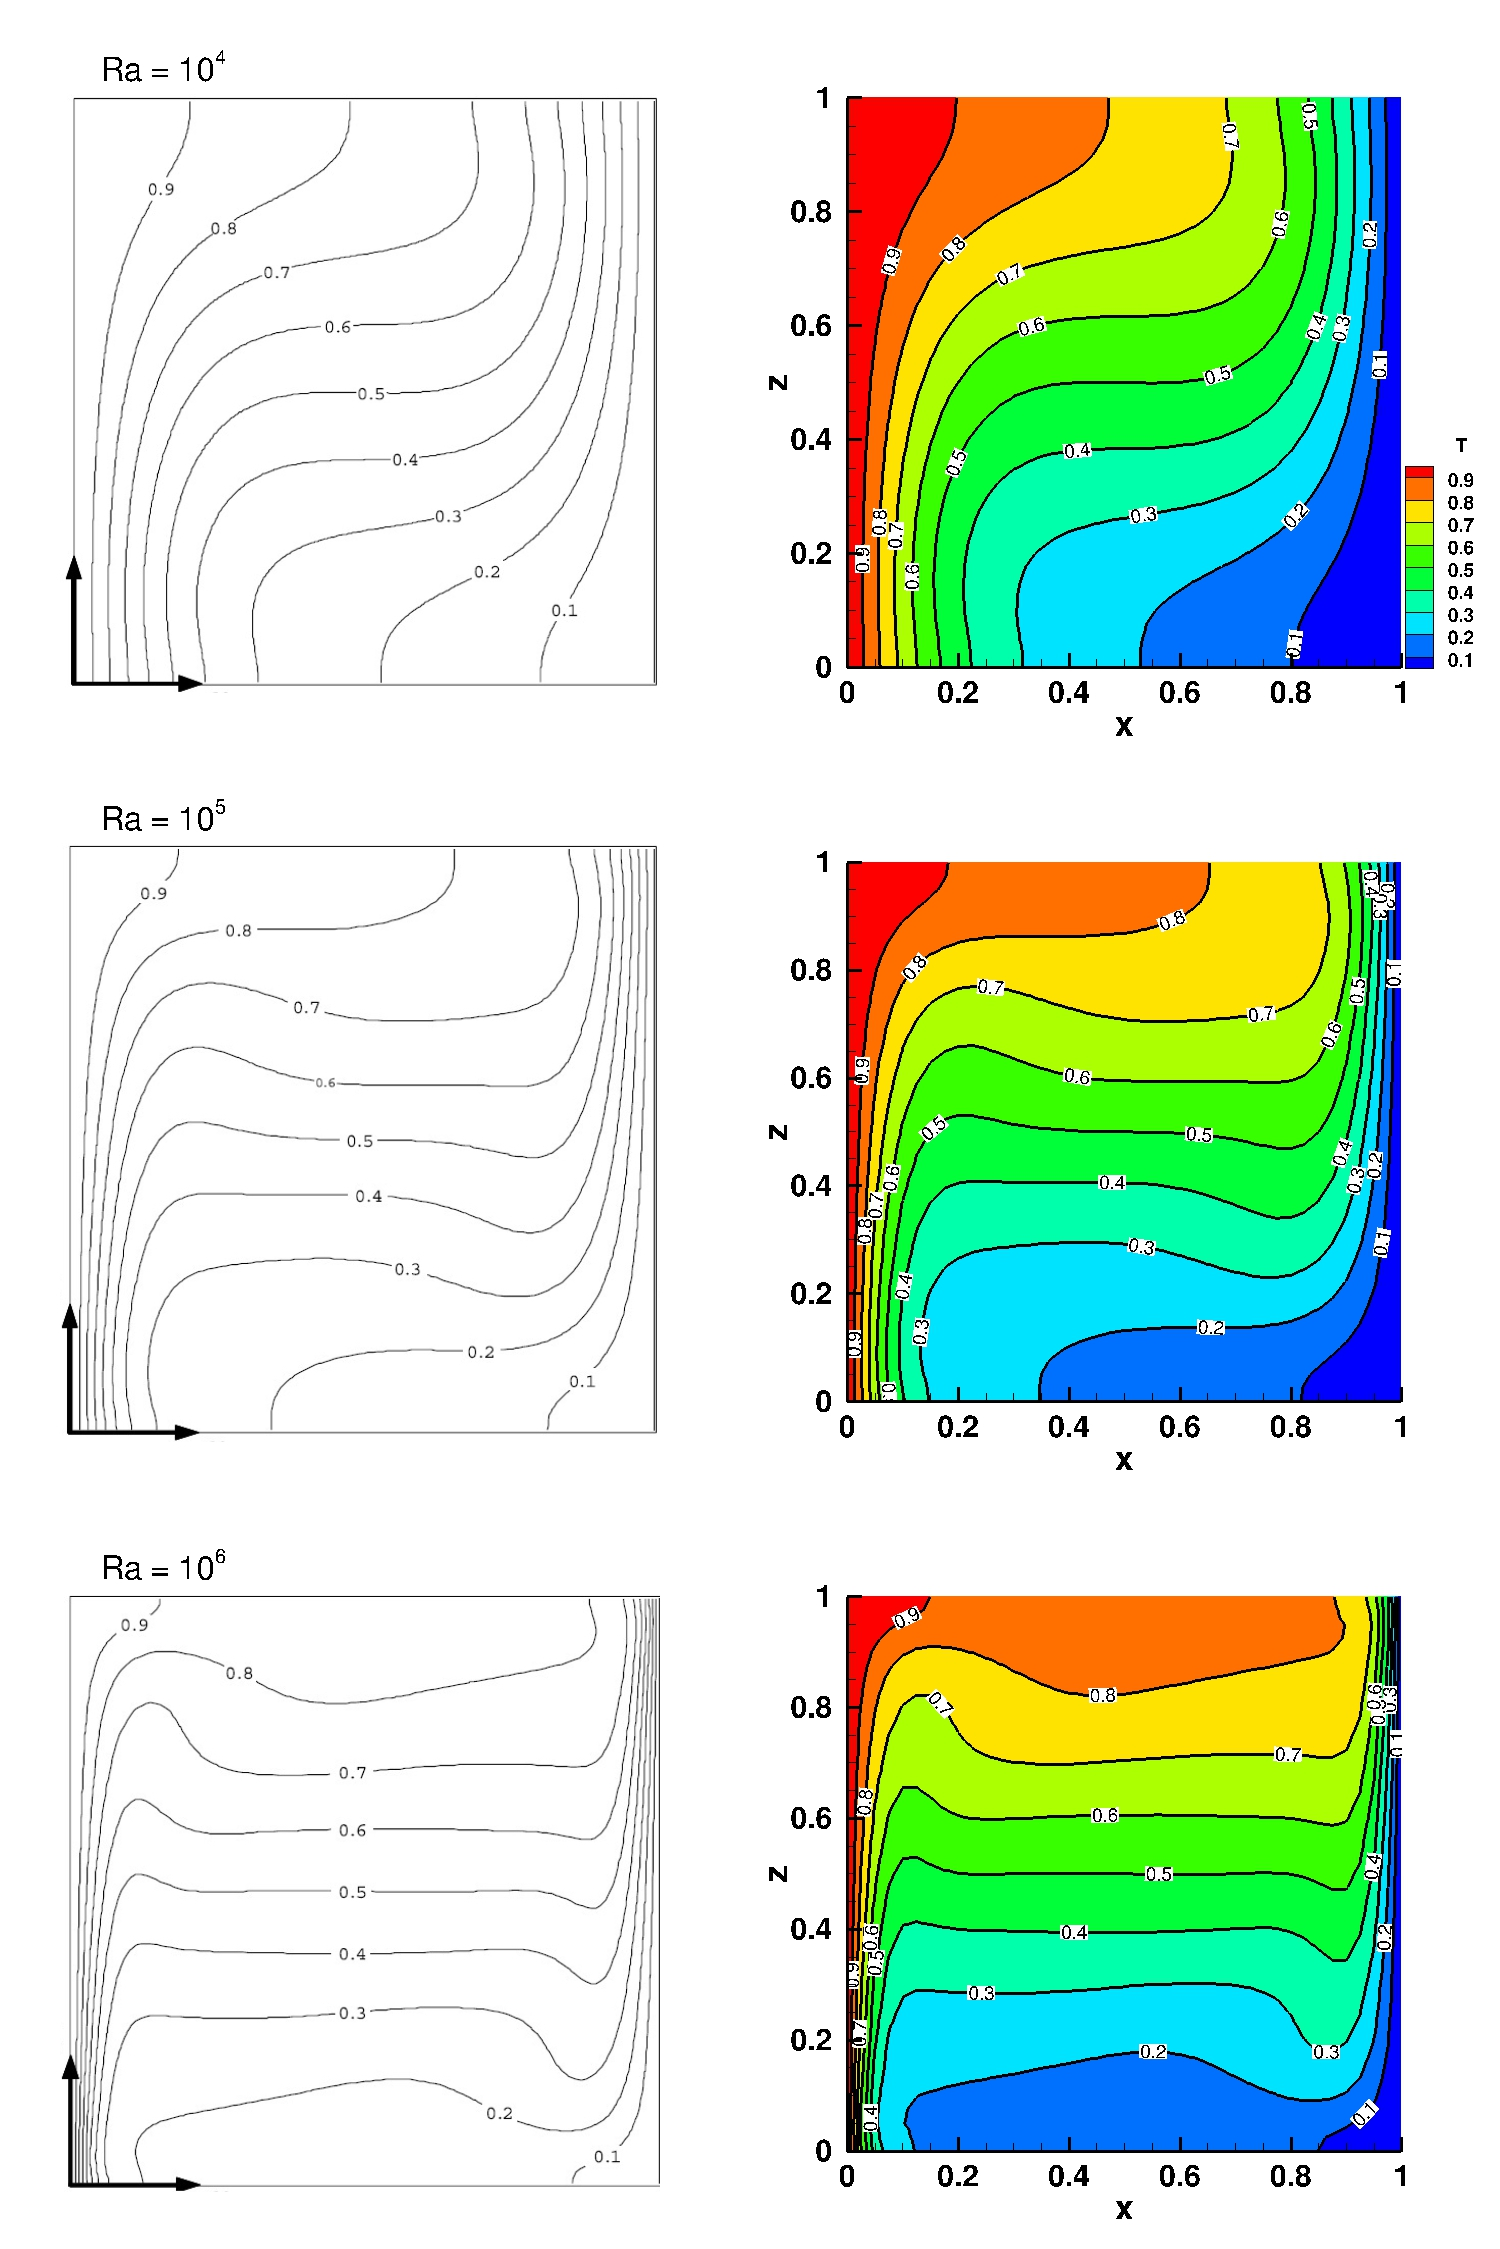
\includegraphics[width=\textwidth]{\figpath/Fig_cap_natconv/Validation_3D_seq_T1}}
%\end{center}
%\end{minipage}
%\caption{3D differentially heated cavity. Temperature contours at the mid-plane of ($y=0.5$); comparison with the results of \cite{Wakashima-2004} (left images). }
%\label{fig-3DT} 
%\end{figure}
%
%\subsection{Natural convection in a cube with an inner heated obstacle}\label{sub-OBSTACLE-3D}
%
%The three-dimensional natural convection induced by a temperature difference between a cold outer cubic enclosure is investigated in this section.
%Sequential and parallel computation using ffddm are carried out and compared together.
%
%Different Rayleigh numbers varying in the range of $10^4 -10^6$ are considered. The temperature field for $Ra = 10^4$ is reported in Figure \ref{fig-obstacle-Ra1e4} and the Table \ref{tab-T2} shows the error between the sequential and the parallel computation.
%
%\begin{figure}%[!htbp]
%\begin{center}
%\begin{minipage}{\linewidth}
% {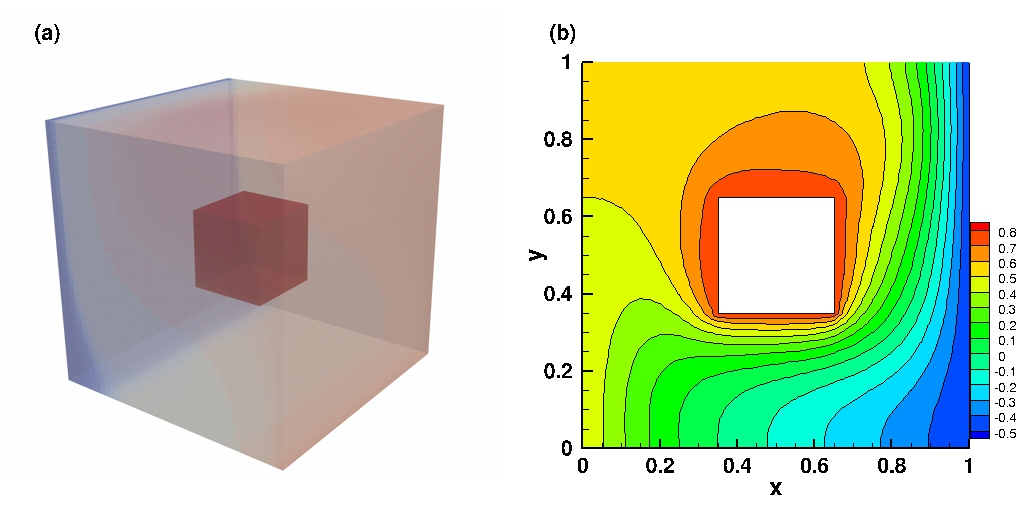
\includegraphics[width=0.98\textwidth]{\figpath/Fig_cap_natconv/3D_OBSTACLE_field}}
%\end{minipage}
%\end{center}
%\caption{3D convection in a cube with an inner heated cube. Temperature fields for $Ra = 10^4$.}
%\label{fig-obstacle-Ra1e4} 
%\end{figure}
%
%\begin{table}[!h]
%	\begin{center}
%		\begin{tabular}{|*{7}{c|}}
%			\hline
%			 Ra & nbseg & nb proc                     & $||u||_{2}$                        & $||u||_{\infty}$                & $||T||_{2}$              & $||T||_{\infty}$\\ \hline \hline
%			\multirow{12}{*}{$10^4$} & \multirow{4}{*}{40} & 28 & $0.00087137$ & $0.0058298$ & $ 0.0022491 $ & $0.01592$ \\
%			\cline{3-7}
%			& & 42 & $0.000870796$ & $0.0058292$ & $ 0.00224866 $ & $0.015921$ \\ \cline{3-7} %\hline 
%			& & 56 & $0.000870646$ & $0.0058293$ & $ 0.00224788 $ & $0.015921$  \\ \cline{3-7} %\hline
%			& & 70 & $0.000870747$ & $0.0058286$ & $ 0.00224795 $ & $0.015921$ \\ \cline{2-7}
%			 & \multirow{4}{*}{60} & 112 & $0.000785593$ & $0.0021$ & $ 0.000858912 $ & $0.010024$ \\% \hline
%			\cline{3-7}
%			& & 140 & $0.000783164$ & $0.002097$ & $ 0.000865668 $ & $0.010024$ \\ \cline{3-7} %\hline 
%			& & 168 & $0.000779419$ & $0.002091$ & $ 0.000858384 $ & $0.010027$  \\ \cline{3-7} %\hline
%			& & 196 & $0.000767662$ & $0.00209$ & $ 0.000864693 $ & $0.010019$ \\ \cline{2-7}
%			 & \multirow{4}{*}{80} & 224 & $0.000637268$ & $0.001795$ & $ 0.000551538 $ & $0.001661$ \\% \hline
%			\cline{3-7}
%			& & 238 & $0.000152936$ & $0.000548$ & $ 0.000205031 $ & $0.000634$ \\ \cline{3-7} %\hline 
%			& & 252 & $0.000239786$ & $0.000841$ & $ 0.000231648 $ & $0.000661$  \\ \cline{3-7} %\hline
%			& & 266 & $0$ & $0$ & $ 0 $ & $0$ \\ \hline 
%			\multirow{12}{*}{$10^5$}& \multirow{4}{*}{40} & 28 & $0.0011359$ & $0.0089746$ & $ 0.00401922 $ & $0.020067$ \\% \hline
%			\cline{3-7}
%			& & 42 & $0.00113742$ & $0.0089788$ & $ 0.00402103 $ & $0.020067$  \\ \cline{3-7} %\hline 
%			& & 56 & $0.00113625$ & $0.0089768$ & $ 0.00402081 $ & $0.020063$   \\ \cline{3-7}%\hline
%			& & 70 & $0.0011348$ & $0.0089726$ & $ 0.00401999 $ & $0.020065$  \\ \cline{2-7} %\hline
%			 & \multirow{4}{*}{60} & 112 & $0.000765582$ & $0.0022345$ & $ 0.00166687 $ & $0.015296$ \\% \hline
%			\cline{3-7}
%			& & 140 & $0.000763449$ & $0.0022313$ & $ 0.00166143 $ & $0.015257$ \\ \cline{3-7} %\hline 
%			& & 168 & $0.000763074$ & $0.0022176$ & $ 0.00166605 $ & $0.015284$  \\ \cline{3-7} %\hline
%			& & 196 & $0.000760368$ & $0.0022093$ & $ 0.00167368 $ & $0.015299$ \\ \cline{2-7} 
%			 & \multirow{4}{*}{80} & 224 & $0.00051462$ & $0.0016627$ & $ 0.000574467 $ & $0.001794$ \\% \hline
%			\cline{3-7}
%			& & 238 & $5.17443 \times 10^{-05}$ & $0.0001934$ & $ 0.00018074 $ & $0.0005666$ \\ \cline{3-7} %\hline 
%			& & 252 & $8.68245 \times 10^{-05}$ & $0.000319$ & $ 8.11788 \times 10^{-05} $ & $0.000335$  \\ \cline{3-7} %\hline
%			& & 266 & $0$ & $0$ & $ 0 $ & $0$ \\ \hline 
%
%		\end{tabular}
%	\end{center}
%	\caption {3D convection in a cube with an inner heated cube. Comparison between sequential and ffddm algorithm for uniform grids of $40 \times 40 \times 40$ for $Ra = 10^4$ and $80 \times 80 \times 80$ for $Ra = 10^5$}
%	\label{tab-T2}
%\end{table}
